\documentclass[a4paper,12pt]{report}
\usepackage[paper=a4paper]{geometry}
\usepackage{placeins}
\usepackage[warn]{mathtext}
\usepackage{graphicx}
\usepackage{amssymb}
\usepackage[justification=centering]{caption}
\usepackage[table,xcdraw]{xcolor}
\graphicspath{{C:\Users\User\Desktop\mipt\phys\lab141}}
\DeclareGraphicsExtensions{.pdf,.png,.jpg}

\usepackage[T2A]{fontenc}
\usepackage[utf8]{inputenc}
\usepackage[english,russian]{babel}
\usepackage{amsmath,amsfonts,amssymb,amsthm,mathtools}
\usepackage{wasysym}
\usepackage{wrapfig}
\author{Выполнил Мещеряков Всеволод, студент Б02-001}
\title{Отчет по лабораторной работе № 1.4.5 \\[15pt] «Изучение колебаний струны»}
\date{\today}

\usepackage{ragged2e}
\justifying


\begin{document}

\maketitle

\section*{Аннотация}

Работа заключается в изучении поперечных стоячих волн на струне: определение собственных частот колебаний струны, исследование зависимости скорости распространения волн на струне в зависимости от ее натяжения. Для этого в работе используются закрепленная на станине струна, набор грузов, электромагнитные датчики, звуковой генератор, двухканальный осциллограф и частотометр.

\section*{Теоритическая справка}

\begin{figure}[h]
	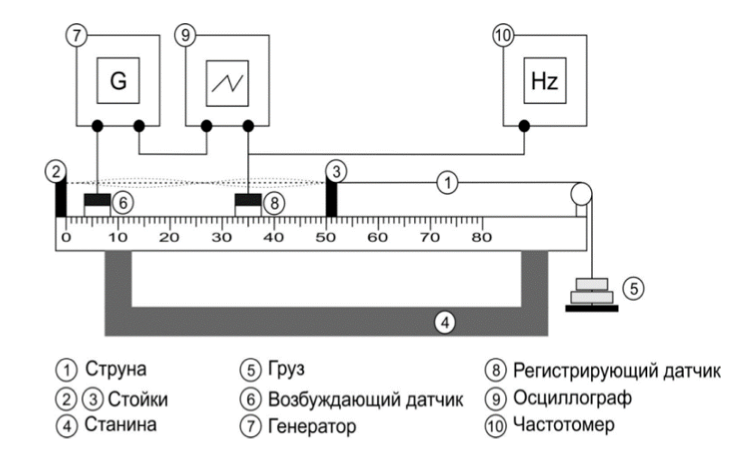
\includegraphics[scale=0.8]{lab145ris1.png}
	\caption{\textit{Схема экспериментальной установки.}}
\end{figure}

На рисунке 1 изображена экспериментальная установка: Струна закреплена между двумя стойками в горизонтальном положении. К одному из концов струны прикреплен груз, создающий натяжение. Возбуждение и регистрация колебаниколебаний струны осуществляются с помощью электромагнитных датчиков (в ибраторов), расположенных на станине под струноструной Возбуждающий датчик подключён к звуковому генератору. Сигнал с
регистрирующего датчика подается на осциллограф.

Основной принцип работы датчиков заключается в том, что участок струны,расположеннырасположенный над э лектромагнитом, совершает колебательное движение в вертикальновертикальной плоскости с частоточастотой генератора. Колебания далее передаются по всей струне и, если частота колебаниколебаний совпадает с одноодной из собственных частот струны, на струне устанавливается стоячая волна. Колеблющаяся струна возбуждает в регистрирующем датчике переменную ЭДС, измеряющуюся с помощью осциллографа.

Струна в акустике - однородная тонкая гибкая упругая нить. Гибкость струны обусловлена тем, что её поперечные размеры малы по сравнению с длиной. Это означает, что напряжение в струне может быть направлено только вдоль неё, что позволяет не учитывать изгибные напряжения, которые могли бы возникать при поперечных деформациях.

Волновое уравнение:

\begin{equation}\label{difur}
	\frac{d^2y}{dt^2}=u\frac{d^2y}{dx^2}
\end{equation}

Где $u$ - скорость распространения волн на струне. Общее решение этого уравнения представимо в виде суммы двух волн произвольной формы, бегущих в противоположные стороны со скоростями $\pm u$.

В случае гармонических волн:

\begin{equation}
	y(x,t)=a\cos{\omega t-kx} + b\cos{\omega t + kx)},
\end{equation}

Где $k=\frac{2\pi}{\lambda}$ - волновое число. Скорость распространения волны же зависит только от силы натяжения и погонной плотности:

\begin{equation} \label{skor}
	u=\sqrt{\frac{T}{p}}.
\end{equation}

Свободные колебания струны с закрепленными концами описываются формулой:

\begin{equation}
	y(x,t)=2a\sin{kx}\cdot\sin{\omega t}.
\end{equation}

Из нее видно, что точки, для которых $\sin{kx}=0$, неподвижны в любой момент времени - их называют узлами. Точки же, для которых $\sin{kx}=1$, называются пучностями. Так как длина волны связана с ее частотой, то струна может колебаться только с определенным набором частот, если на длине струны укладывается целое число полуволн:

\begin{equation} \label{chast_n}
	\nu_n=\frac{n}{2L}\sqrt{\frac{T}{\rho}}.
\end{equation}

Набор разрешенных частот $\nu_n$ называют собственными частотами колебаний струны. Наименьшая частота $\mu_1$ называется также основным тоном (или первой гармоникой), а остальные - обертонами (высшими гармониками). 

\section*{Работа с установкой}

\subsection*{Измерения}

Прежде чем приступить к измерениям, стоит убедиться, что возбуждающий датчик расположен вблизи неподвижного конца струны, а регистрирующий - вблизи пучности. 

\subsubsection*{Регистрация стоячих волн с помощью осциллографа}

В этой части работы мы будем измерять гармоники для разных нагрузок. Измерим массы и рассчитаем нагрузки - результаты приведем в \textbf{таблице 1.}

Визуально настроим струну на основную гармонику, не меняя ее нагрузку и длину. Регистрирующий датчик установим в центре под струной. 

Подстроим частоту $\nu$ генератора так, чтобы амплитуда сигнала была максимальна. Добьемся отсутствия нелинейных искажений, уменьшая амплитуду напряжения генератора, и при этом подстраивая частоту так, чтобы она соответствовала максимуму сигнала. Запишем окончательное значение частоты основной гармоники $\nu_1$. Проведем измерения частот для нескольких нечетных гармоник стоячих волн при длине струны 50 см и массе грузов $\approx$ 1 кг. Измерим частоты гармоник. Для этого станем смещать регистрирующий датчик 8 в предварительные расположения пучностей. Результаты занесем в \textbf{таблицу 2.}

\subsection*{Обработка результатов}

Сравним значения частот $\nu_n$, полученных при визуальном наблюдении и наблюдении с помощью осциллографа:

По \textbf{таблице 2} построим графики зависимостей частоты $\nu_n$ от номера $n$ гармоники для различных натяжений $T$ - \textbf{рисунок 2}. По ним определим скорости волн $u$ и оценим погрешность.

На основании коэффициентов наклона получим \textbf{таблицу 3} со скоростями для каждой из нагрузок.

Построим график зависимости квадрата скорости $u^2$ от силы натяжения $T$ по имеющимся данным - \textbf{рисунок 3}. Из них определим погонную плотность струны $\rho_l$.

Из графика зависимости квадрата скорости волны от величины нагрузки получим коэффициент наклона прямой $k=1764,9 (м/кг) $  с точностью $\pm 9,3 \cdot 10^-6 м/кг$. Тогда определим погонную плотность струны - она равна величине обратной значению коэффициента наклона прямой:

\begin{equation}
	\rho = 566 \pm 9 мг/м
\end{equation}

Установим частоту $\nu_1/2 \approx 45.3 Гц$ для первой нагрузки. Переключим осциллограф на режим X-Y. На экране увидим фигуру Лиссажу с одним самопересечением - это как раз говорит об отношении частот 2:1 - \textbf{Рисунок 4}. 


\section*{Приложение - графики и таблицы.}

\begin{table}[h!]
\centering
\begin{tabular}{|c|c|c|c|c|c|}
\hline
\cellcolor[HTML]{FFFFFF}\textbf{\begin{tabular}[c]{@{}c@{}}Массы \\ грузов, г\end{tabular}} & 462   & 941.5  & 1423   & 1915.8 & 2409.3 \\ \hline
\textbf{Нагрузки, Н}                                                                        & 5.686 & 10.390 & 15.113 & 19.948 & 24.789 \\ \hline
\end{tabular}
\caption{\textit{Изучаемые нагрузки. В массе каждого груза необходимо добавлять массу подвеса - 117.6 грамм.}}
\end{table}

\begin{table}[h!]
\centering
\scalebox{0.9}{
\begin{tabular}{|c|c|c|c|c|c|}
\hline
\cellcolor[HTML]{FFFFFF}\textbf{\begin{tabular}[c]{@{}c@{}}Величина   нагрузки, Н\\      / Номера гармоник\end{tabular}} & \textbf{5.7} & \textbf{10.4} & \textbf{15.1} & \textbf{19.9} & \textbf{24.8} \\ \hline
\textbf{1 Гармоника, Гц}                                                                                                 & 99.95        & 143.41        & 163.85        & 193.5         & 208.8         \\ \hline
\textbf{2 Гармоника, Гц}                                                                                                 & 198.7        & 283.1         & 325.7         & 384.4         & 413.8         \\ \hline
\textbf{3 Гармоника, Гц}                                                                                                 & 301.4        & 429.6         & 491.1         & 578.8         & 628.8         \\ \hline
\textbf{4 Гармоника, Гц}                                                                                                 & 399.5        & 569.2         & 653.2         & 772.7         & 836.6         \\ \hline
\textbf{5 Гармоника, Гц}                                                                                                 & 501.3        & 715.6         & 810.4         & 964.6         & 1050.5        \\ \hline
\textbf{6 Гармоника, Гц}                                                                                                 & 602.4        & 858.7         & 981.9         & 1157.8        & 1253.8        \\ \hline
\textbf{7 Гармоника, Гц}                                                                                                 & 698.3        & 1002.3        & 1144.2        & 1353.3        & 1463.9        \\ \hline
\textbf{8 Гармоника, Гц}                                                                                                 & 798.7        & 1144.9        & 1311.1        & 1544.9        & 1673.2        \\ \hline
\textbf{9 Гармоника, Гц}                                                                                                 & 897.2        & 1286.7        & 1470.9        & 1738.9        & 1877.9        \\ \hline
\textbf{10 Гармоника, Гц}                                                                                                & 997.8        & 1429.8        & 1634.7        & 1931.4        & 2090.4        \\ \hline
\end{tabular}
}
\caption{\textit{Измеренные гармоники для каждой из нагрузок.}}
\end{table}


\begin{figure}[h!]
	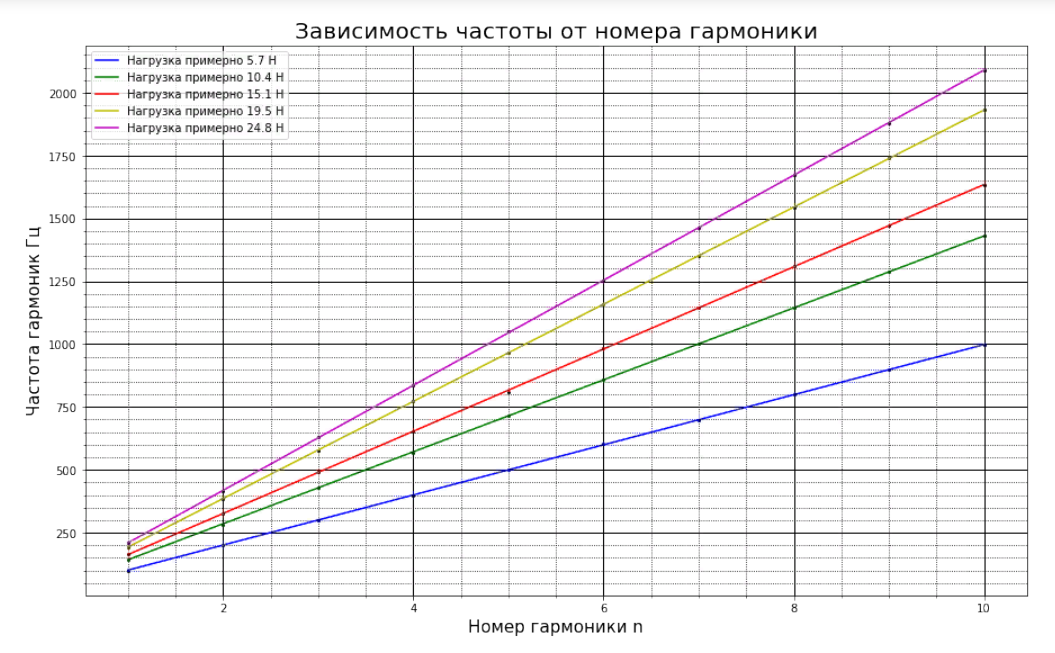
\includegraphics[scale=0.7]{lab145ris2.png}
	\caption{\textit{Зависимость частоты гармоники от ее номера для разных нагрузок.}}
\end{figure}

\begin{table}[h!]
\centering
\scalebox{0.7}{
\begin{tabular}{|c|c|c|c|c|c|}
\hline
\textbf{Величина   нагрузки, Н}                                                                             & 5.69       & 10.39       & 15.11       & 19.95       & 24.79       \\ \hline
\cellcolor[HTML]{FFFFFF}\textbf{\begin{tabular}[c]{@{}c@{}}Коэффициенты\\ наклона {[}Гц{]}\end{tabular}}    & 99.67      & 143.11      & 163.22      & 193.22      & 208.96      \\ \hline
\textbf{\begin{tabular}[c]{@{}c@{}}Погрешность\\ вычисления\\ коэффициента\\ наклона {[}Гц{]}\end{tabular}} & 0.07621467 & 0.072463754 & 0.128123212 & 0.047079382 & 0.127711673 \\ \hline
\textbf{\begin{tabular}[c]{@{}c@{}}Скорость волны\\ {[}м/c{]}\end{tabular}}                                 & 99.67      & 143.11      & 163.22      & 193.22      & 208.96      \\ \hline
\end{tabular}
}
\caption{\textit{Скорость волны при разных нагрузках.}}
\end{table}

\begin{figure}[pt!]
	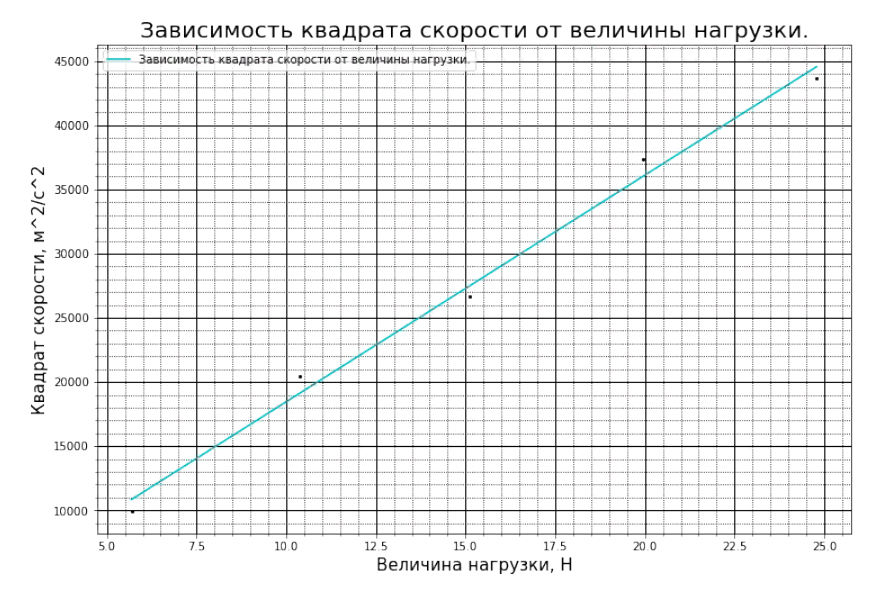
\includegraphics[scale=0.8]{lab145ris3.png}
	\caption{\textit{Зависимость квадрата скорости волны от величины нагрузки.}}
\end{figure}

\begin{figure}[pt!]
	\centering
	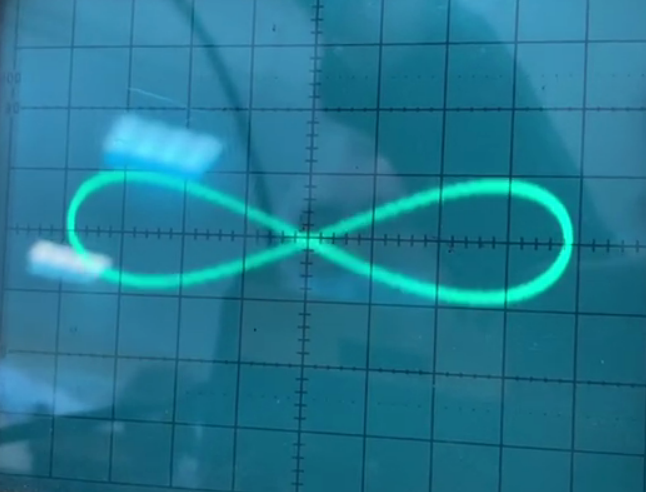
\includegraphics[scale=0.8]{lab145ris4.png}
	\caption{\textit{Фигура Лиссажу.}}
\end{figure}

\end{document}